Ultimately, we will design a deterministic finite automaton (DFA) $M = \langle Q, \Sigma, \delta, q_0, F \rangle$, where $Q$ is the state set, $\Sigma$ is the input alphabet, $\delta : Q\times\Sigma \rightarrow Q$ is the transition function, $q_0$ is the initial state, and $F\subseteq Q$ is the set of final states.

First, we define the alphabet $\Sigma$. A finite lattice is represented as a sequence of 5-bit binary strings as described in Figure~\ref{fig:encoding-symbol}. We encode the lattice left-to-right. Note that this means for the first (leftmost) symbol $a=a_0a_1a_2a_3a_4$, it must be the case that $a_0 = a_2 = a_4 = 0$, because edges that correspond to these three symbols do not appear on the lattice.

\begin{figure}
\begin{center}
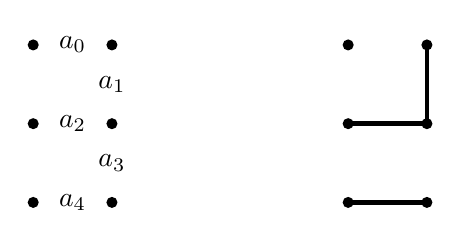
\begin{tikzpicture}
\foreach \x in {0,1}
\foreach \y in {0,1,2}
{
\fill (\x,\y) circle (2pt);
}
\node at (0.5,2) {$a_0$};
\node at (1,1.5) {$a_1$};
\node at (0.5,1) {$a_2$};
\node at (1,0.5) {$a_3$};
\node at (0.5,0) {$a_4$};

\foreach \x in {4,5}
\foreach \y in {0,1,2}
{
\fill (\x,\y) circle (2pt);
}
\draw [ultra thick] (5,2) -- (5,1) -- (4,1);
\draw [ultra thick] (4,0) -- (5,0);
\end{tikzpicture}
\end{center}
\caption{\emph{Left:} Positions of each of 5 bits in the binary string $a = a_0a_1a_2a_3a_4$, a symbol in the alphabet; $a_i = 1$ if there is an edge in position $a_i$, and 0 otherwise. \emph{Right:} Example input symbol $a=01101$ as it appears on the lattice.}
\label{fig:encoding-symbol}
\end{figure}

The finite automaton reads input symbols over the alphabet described above, and determines if they represent a valid self-avoiding walk as defined in Section~\ref{sec:statement}. A state in this automaton is represented by a 4-tuple $q = \langle t, m, b, c\rangle$:
\begin{itemize}
\item Elements $t$, $m$, and $b$ represent the degrees of the top, middle, and bottom (respectively) of the rightmost vertices of the input so far. (Notice that these values depend only on the most recent input symbol.) Because self-avoiding walks do not have branches, we are only interested in states for which $t, m, b \in \{0, 1, 2\}$. Provided the input is a valid walk, the number of ones among $t$, $m$, and $b$ represents the number of vertices that the next input symbol may connect to. We divide states by this characteristic:
\begin{itemize}
\item If a state has a single 1-degree vertex, then we refer to it as \emph{single-ended}.
\item If a state has exactly two 1-degree vertices, then we refer to it as \emph{double-ended}. Notice that if we are in a double-ended state, we must have already seen both ends of the valid walk (because one end is at the origin and to induce a second would otherwise require a branch, which is not allowed).
\item If a state has three 1-degree vertices, then we refer to it as \emph{triple-ended}. For the purpose of identifying closed loops, we require an additional bit of state in the case of triple-ended states because two possible pairs of states may have already been connected; see the description of the $c$ element.
\item If a state has no 1-degree vertices, then we have finished processing the walk and any further input should be trivial in order for the lattice to be valid.
\end{itemize}
\item Element $c$ represents closure information. If the state is single- or double-ended, then $c$ is not needed (so $c=0$ in those cases); if the state is triple-ended, $c$ will be either 1 or 2 depending on which pair of vertices is connected:
\begin{itemize}
\item If the top and middle vertices are connected, then $c=2$.
\item If the middle and bottom vertices are connected, then $c=1$.
\end{itemize}
\end{itemize}

In addition to the states that can be described in the manner outlined above, we will use three auxilliary states: \emph{`start'}, \emph{`done'}, and \emph{`dead'}. We present the complete list of required states in Table~\ref{tab:states}.

\begin{table}
\begin{center}
\begin{tabular}{cccc}
\hline
Single-ended & Double-ended & Triple-ended & Auxilliary \\
\hline
1000 & 1010 & 1111 & \emph{start} \\
1200 & 1210 & 1112 & \emph{done} \\
1220 & 1100 &  & \emph{dead} \\
0100 & 1120 &  &  \\
2100 & 0110 &  &  \\
0120 & 2110 &  &  \\
0010 &  &  &  \\
0210 &  &  &  \\
2210 &  &  &  \\
\hline
\end{tabular}
\end{center}
\caption{All states of interest, categorized by how many 1-degree vertices there are in the set of rightmost vertices. Final states include all the single-ended states, as well as the \emph{`start'} (accept walks of length 0), and \emph{`done'} states.}
\label{tab:states}
\end{table}
